\chapter{Arquitectura}

El sistema modular para la adquisición, gestión y visualización web de métricas de desempeño, está compuesto por cuatro capas cada una con una funcion especifica dentro de la representación y gestión de las métricas de desempeño que se presentan al usuario.

Los componentes del SMMD se clasifican de la siguiente manera:
\begin{enumerate}
	\item Recolectores de métricas
    \begin{enumerate}
    \item Collectd, un proceso que se ejecuta en segundo plano a nivel del nodo en donde se ejecutan los algoritmos o el procesamiento de datos, el cual se encarga de tomar todas las métricas de desempeño a través de plugins que se activan en un archivo de configuración.
    \item Metricbeat, un proceso que se ejecuta en segundo plano a nivel del nodo en donde se ejecutan los algoritmos o el procesamiento de datos el cual toma metricas básicas del sistema operativo y las envia al recolector de logs.
    \end{enumerate}
    \item Recolector de Logs
	\begin{enumerate}
      \item Logstash, es un proceso se ejecuta en el servidor, en este caso en el equipo que utiliza el investigador al cual los nodos envian la información de métricas de desempeño.
    \end{enumerate}
    \item Persistencia de Datos
    \begin{enumerate}
      \item Elastic Search, representa la capa de persistencia de datos y procesamiento, una vez la información ha sido recibida desde Logstash, elastic search se encarga de procesar y persistir la información en un formato de documento de typo JSON \footnote[1]{JavaScript Object Notation, un formato de intercambio de datos basado en el estándar ECMA-262 del lenguaje de programación Javascript}
    \end{enumerate}
    \item Presentación
    \begin{enumerate}
      \item Kibana, es un visualizador de datos, que permite explorar la información que se encuentra en Elastic Search y provee herramientas de fácil uso para la creación de paneles de control y vistas generales para la visualización de métricas de desempeño. Utiliza los paneles de control pre-definidos por metric beat para representar el uso de recursos tales como memoria, procesador y almacenamiento con actualizaciones en tiempo real.
    \end{enumerate}
\end{enumerate}

Tal como se puede observar en la figura \ref{fig:modelo-sistema} SMMD está modelado en una arquitectura de tipo cliente/servidor en donde el cliente está representado por los nodos que son asignados en el cluster al investigador para que este utilice sus recursos en la ejecución de programas o procesamiento de datos. El administrador provee de manera transparente al investigador dichos nodos con sistema operativo previamente instalado, que en el caso particular de este proyecto y acorde a los proyectos que se manejan actualmente en el CECAD, es un sistema operativo Linux en alguna de las dos distribuciones CentOS 7 o Ubuntu Xenial 16.04.
\\\\
Todo nodo que sea monitoreado utilizando SMMD, contiene dos colectores de métricas Collectd y Metric beat respectivamente los cuales envian información al servidor central, el cual está bajo el control de investigador y en donde se encuentran los componentes de recolección de logs, persistencia de datos y visualización. A partir de configuraciones específicas para el recolector de métricas Collectd, el investigador está en la capacidad de incluir diferentes plugins que le permitirán visualizar diferentes tipos de métricas de acuerdo a su necesidad particular. A nivel del servidor que como bien se menciono anteriormente está bajo el control del investigador, los componentes de recolección de logs, persistencia de datos y presentación, están aislados del sistema de archivos del sistema operativo y corren en un espacio de usuario alterno gracias al uso de contenedores Docker que están orquestados utilizando la herramienta docker-compose\footnote{https://docs.docker.com/compose, Compose es una herramienta para definir y correr aplicaciones de múltiples contenedores en Docker}, los cuales no tienen dependencia directa las librerias o software del sistema operativo permitiendo así la operabilidad en distintos sistemas operativos que soporten la tecnología Docker, tales como MacOS, Windows y Linux en distintas arquitecturas de procesador como los son x86, amd64, ARM, ppc64le (IBM Power) y s390x (IBM Z). Adicionalmente como consecuencia de la independencia de estos componentes con librerias propias del sistema operativo, permite que la instalación sea mucho más sencilla para el investigador sin la necesidad que este tenga que preocuparse por instalar dependecias en su sistema, con la simple instalación de Docker el investigador tendrá a su disposición el componente del servidor sin inconveniente alguno.

A continuación de presentará en detalle cada uno de los componentes de las capas de SMMD en donde se mencionará en detalle la interoperatibilidad entre dichas tecnologías que permite el funcionamiento de SSMD.

\begin{figure}
 \centering
  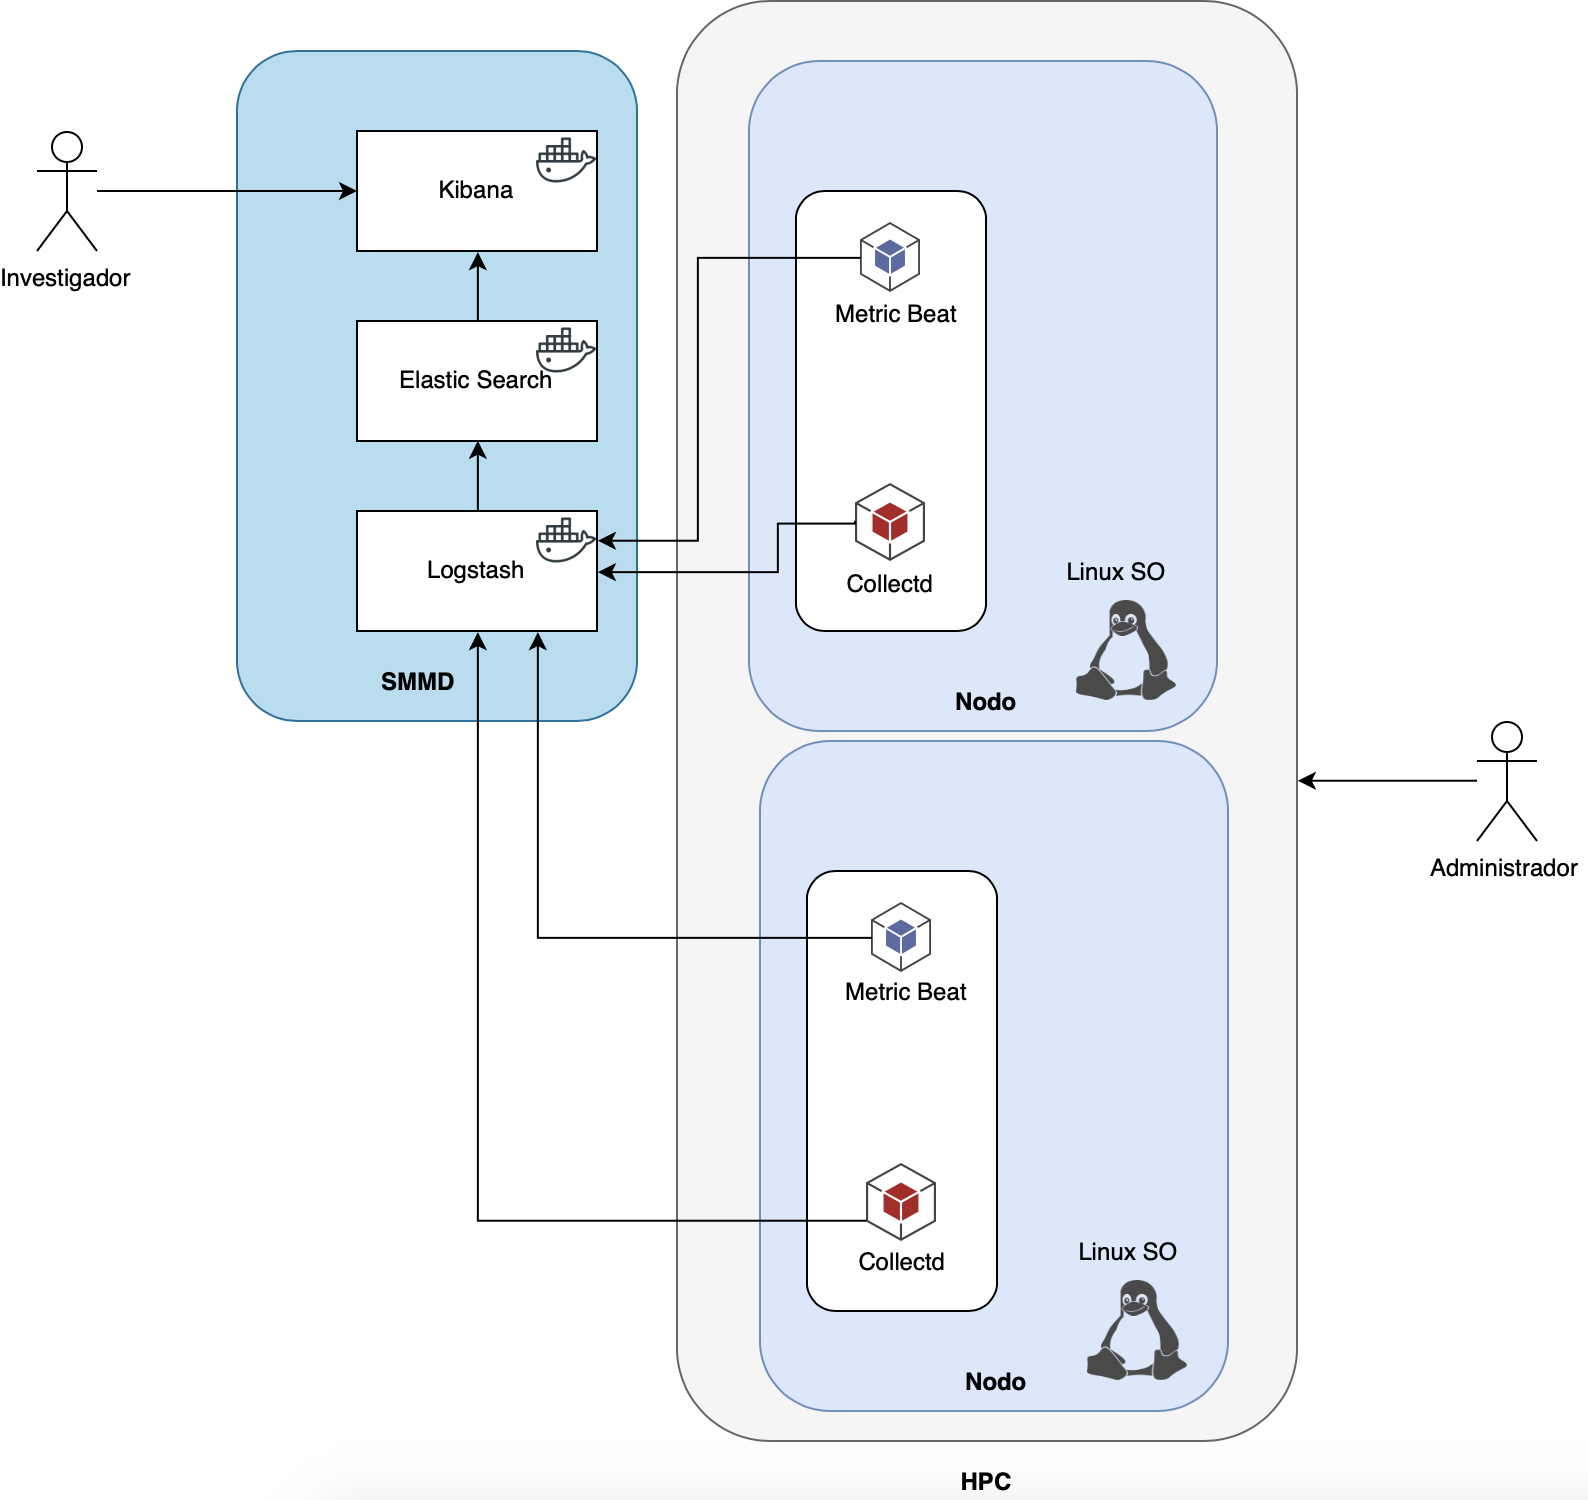
\includegraphics[width=0.9\linewidth]{./imagenes/arquitectura-general.png}
  \caption{Modelo General del Sistema SMMD.}
  \label{fig:modelo-sistema}
\end{figure}


\newpage

\section{Recolección de Métricas}



\subsection{Tipos de Métricas}

En el espacio del tipo de métricas que SMMD soporta actualemente se suman los dos grandes conjuntos de métricas que provee el sistema a través de las herramientas Metricbeat y Collectd, cada uno es una tecnología separada e independiente con propositos e implementación complementamente distintos los cuales se describen a continuación.

Las métricas soportadas son 


\subsection{Metricbeat}\label{metricbeat}
Metricbeat\footnote[1]{https://www.elastic.co/products/beats/metricbeat} conocido también como Elastic Metricbeat, hace parte de la suite de herramientas de Elastic\footnote[2]{Elastic NV, compañía Europea fundada por Shay Banon en 2012 conocida antiguamente como Elasticsearch, es una una compañía dedicada a ofrecer servicios de tipo SaaS (Software como servicio) para el análisis y búsqueda de logs principalmente, servicios usados por compañías reconocidas como: eBay, Cisco, Microsoft y la NASA).} es un software que corre como servicio o demonio el cual permite procesar métricas de desempeño básicas como: uso de CPU, carga promedio del sistema, memoria, uso de red y lecto-escritura en disco. 
Provee la capacidad de habilitar módulos para procesar métricas de otros sistemas como HAProxy, Apache Kafka, Kubernetes, MongoDB, MySQL entre otros. Debido a que su instalación es muy sencilla y su integración con otros productos de la misma compañía es buena, es la opción estandar para la obtención de métricas básicas de desempeño.



\subsection{Collectd}\label{demonio-collectd}
Existen diversos tipos de software para la recolección de métricas de desempeño, para el caso particular de este proyecto se utilizará \textbf{Collectd}, un software de tipo demonio\footnote[3]{Un programa de computadora que corre como un proceso en segundo plano el cual no está bajo el control directo del usuario actual del sistema}, 

\subsection{Statsd}\label{statsd}
Statsd es un demonio de muy facil uso



\section{Gestión de Métricas}
Logstash es un motor de procesamiento y recopilación de datos basado en plugins. Incluye una gran variedad de plugins que permiten configurarlo fácilmente para recopilar, procesar y reenviar datos en muchas arquitecturas diferentes. \hl{Registrar fuente y actualizar}

El procesamiento se organiza en uno o más pipelines. En cada pipeline, uno o más plugins de entrada reciben o recopilan datos que luego se colocan en una cola interna. De manera predeterminada, esta es pequeña y se almacena en la memoria, pero puede configurarse para ser más amplia y permanecer en el disco para mejorar la confiabilidad y la persistencia.

Los hilos de procesamiento leen datos de la cola y los procesan a través de cualquier plugin de filtro configurado en secuencia. Logstash viene de fábrica con una gran cantidad de plugins destinados a tipos específicos de procesamiento, y así es como se analizan, procesan y enriquecen los datos.

Una vez que se procesan los datos, los hilos de procesamiento envían los datos a los plugins de salida correspondientes, que son los responsables de formatear y enviar los datos hacia adelante, por. ej., a Elasticsearch.

Los plugins de entrada y salida también pueden tener un plugin de códec configurado. Esto permite formatear datos antes de colocarlos en la cola interna o antes de enviarlos a un plugin de salida.


\section{Persistencia}
Elasticsearch es un motor de búsqueda basado en Lucene. Lucene es una API gratuita y de código abierto para hallar informaciones y se usa mucho para crear motores de búsqueda.

Elasticsearch, a través de interfaces web HTTP y documentos JSON, permite interactuar de forma sencilla con su núcleo y realizar búsquedas de texto completo muy eficaces.

La misión de Elasticsearch parte de una convicción de Shay Banon, el fundador: “Search is something that any application should have”. Basándose en este credo, Banon trabajó durante años para llevar su compañía a la cima de la escena informática mundial.

Hoy Elasticsearch es un sistema distribuido que escala horizontalmente, basado en nodos que a su vez se dividen en clústeres. La comunicación hacia y desde los clústeres se realiza a través de las REST API que utilizan HTTP. Las aplicaciones de los clientes que utilizan este proyecto se pueden escribir en cualquier lenguaje. La arquitectura subyacente es obviamente invisible para el usuario, que percibe todo como una entidad única, aunque la naturaleza distribuida de la pila hace que los procesos se interconecten entre sí a través de un intercambio continuo de mensajes entre los nodos. Estos últimos tienen tareas muy específicas que se dividen en autonomía, dependiendo de las configuraciones que se le da a los distintos balances de carga. Si los recursos establecidos al principio no son suficientes, Elasticsearch puede “ampliar” su capacidad de procesamiento activando nuevos nodos y creando nuevos clústeres, con total autonomía; de aquí su naturaleza escalable.
 
\newpage

\section{Comunicación}

\section{Protocolos de operabilidad}
Aqui que protocolo utiliza logstash, collectd y metric beat.


\subsection{Operabilidad en Red}
En el aspecto de la comunicación entre cliente y servidor, SMMD permite dos configuraciones básicas como se puede observar en la figura \ref{fig:modelo-comunicacion} 

\begin{enumerate}
	\item Usuario externo: En este escenario el investigador se encuentra en un red externa fuera del rango IPs accesible necesario para que las másquinas virtuales asignadas por el administrador envien información periodica al servidor. La linea roja en el diagrama \ref{fig:modelo-comunicacion} representa el flujo de la información desde el interior de la red del centro de computo hasta el servidor principal SMMD controlado por el investigador. Para este escenario, el investigador deberá solicitar al administrador del HPC acceso a la red interna a través de un VPN con el fin de establecer una LAN virtual entre los nodos asignados en el cluster y el equipo servidor que recibira el reporte de las métricas de desempeño.
	\item Usuario interno: En este escenario el usuario se encuentra físicamente en la LAN del centro de computo, y comparte una misma subred lo cual hace que los nodos asignados vean la dirección ip del servidor y puedan enviar la información de métricas de desempeño.
\end{enumerate}
Como se mencionará en el capítulo de instalación, los valores de red a configurar en los nodos son dinámicos y permiten ajustarse a cualquier de los dos escenarios mencionados anteriormente.

\begin{figure}[h]
 \centering
  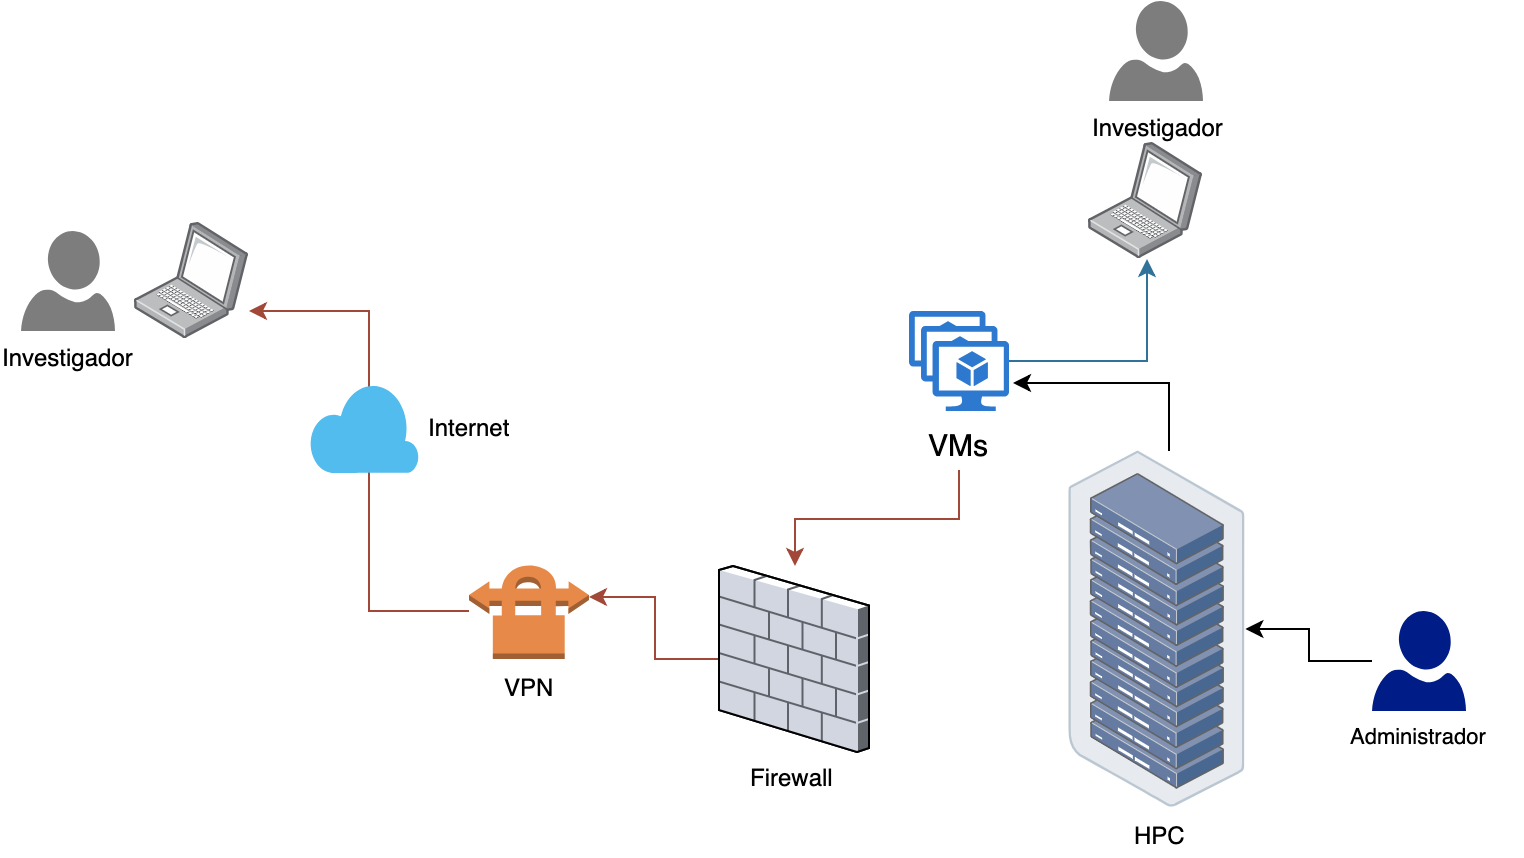
\includegraphics[width=0.9\linewidth]{./imagenes/comunicacion.png}
  \caption{Comunicacion Cliente - Servidor.}
  \label{fig:modelo-comunicacion}
\end{figure}
\newpage
\section{Visualización}
Kibana es una plataforma de análisis y visualización de código abierto diseñada para trabajar con Elasticsearch. Utiliza Kibana para buscar, ver e interactuar con datos almacenados en los índices de Elasticsearch. Puede realizar análisis de datos avanzados y visualizar fácilmente sus datos en una variedad de gráficos, tablas y mapas.

Kibana facilita la comprensión de grandes volúmenes de datos. Su sencilla interfaz basada en navegador le permite crear y compartir rápidamente paneles dinámicos que muestran cambios en las consultas de Elasticsearch en tiempo real.

La configuración de Kibana es muy fácil. Puedes instalar Kibana y comenzar a explorar sus índices Elasticsearch en minutos - sin código, sin infraestructura adicional requerida.

